\section{Syntax of \GRust}
\label{sec:grust:syntax}

The \GRust language, whose syntax is depicted in EBNF notation in \Cref{fig:syntax:grust}, is
composed of three elements: the service-modeling kernel \GRFRP used to define computations on flows
and their interaction with the system; the reactive library \GReact that offers built-in operators
on flows; and the component-modeling kernel \GRSync for user-defined operators on flows. Items from
those elements are recorded in a program (Program).

\begin{figure}[!ht]
    \centering
    \begin{bnf}(comment = {:is:})
        \Prog ::= \many{\Item} ;;
        \Item ::= \InterItem // \ServItem // \FunItem // \CompItem ;;
        \TY   ::= \boolTY // \intTY // \floatTY // \unitTY ;;
    \end{bnf}
    \caption[EBNF grammar of \GRust.]%
    {
        EBNF grammar of \GRust, composed of three elements: the service-modeling kernel \GRFRP, the reactive
        library \GReact, and the component-modeling kernel \GRSync.
        Repetitions of \texttt{X} are denoted \many{\texttt{X}}.
    }
    \label{fig:syntax:grust}
\end{figure}

Although the implemented prototype enables array and user-defined types like enumerations and
structures, in this syntax, types (\TY) are limited to \boolTY, \intTY, and \floatTY.

\subsection{Syntax of \GRFRP}
\label{sec:grust:syntax:grfrp}

This section presents the syntax of \GRFRP, depicted in EBNF notation in \Cref{fig:syntax:grfrp}.
It combines the declaration of services, entities that computes data flows, and their interaction
with the real system \via an interface. Inspired from the \frp paradigm, \GRFRP defines flow
computation in a declarative style.

\begin{figure}[!ht]
    \centering
    \begin{bnf}(comment = {:is:})
        \InterItem ::= \importX{\typed{\FlowKind}{\ID}{\TY}} // \exportX{\typed{\FlowKind}{\ID}{\TY}} ;;
        \ServItem ::= \servItem{\ID}{\interval{\INT}{\INT}}{\many{\FlowStmt}} ;;
        \FlowStmt ::= \letStmt{\many{(\typed{\FlowKind}{\ID}{\TY})}}{\FlowOp} // \defStmt{\many{\ID}}{\FlowOp} ;;
        \FlowOp ::= \ID // \compApp{\ID}{\many{\FlowOp}} // \GReactExpr ;;
        \FlowKind ::= \signalKind // \eventKind ;;
    \end{bnf}
    \caption[EBNF grammar of \GRFRP.]%
    {EBNF grammar of \GRFRP.
        Terminal symbols are in purple.
        Repetitions of \texttt{X} are denoted \many{\texttt{X}}.
        \ID are identifiers composed of ASCII characters.
        \INT is an integer.}
    \label{fig:syntax:grfrp}
\end{figure}

In \GRFRP, data flows are categorized as \emph{signals} for continuous values and \emph{events} for
discrete occurrences. The value of a signal is always available but may change over time, while
events values are only accessible when they occur.

The interface is declared by \emph{imports} and \emph{exports} of flows (InterfaceDecl):
the imported flows are produced by other entities in the system (sensors, or other services);
the exported flows are produced by the program and made available for other entities in the system
(actuators, or other services).

A service is a unique instantiation of flow computations. Its declaration names the service, states
timing constraints (\kft{@}\interval{\INT}{\INT}), and provides the ordered list of flow
statements (\block{\many{\FlowStmt}}) that defines the behavior of the service. As explained in
\Cref{sec:grust:example}, services are not periodic, but follow time constraints, ensuring that new
values are published between a minimum and maximum delay.

Flow statements are of two kinds: declarations (\letStmt{\many{(\typed{\FlowKind}{\ID}{\TY})}}
{\FlowOp}) define the behavior of local flows; definitions (\defStmt{\many{\ID}}{\FlowOp}) state
the values of exported flows. A single service and a single declaration can define an exported flow,
but this can only be verified locally and not system-wide.

Signals and events are defined by flow operations composed of identifiers (\ID), operations from
the \GReact library (\GReactExpr), and calls of flow operators defined in the \GRSync kernel
(\compApp{\ID}{\many{\FlowOp}}). Both \GReact and \GRSync are described in
\Cref{sec:grust:syntax:greact,sec:grust:syntax:grsync} respectively.

\subsection{Syntax of \GReact}
\label{sec:grust:syntax:greact}

Inspired by ReactiveX~\cite{reactivex}, \GReact is a library that extends \GRFRP by offering
built-in operators on flows. The syntax of \GReact operators is presented in
\Cref{fig:syntax:greact}, and \Cref{fig:greact_operators} illustrates their behaviors.

\begin{figure}[!ht]
    \centering
    \begin{bnf}(comment = {:is:})
        \GReactExpr ::= \onchangeExpr{\FlowOp} //  \persistExpr{\FlowOp}
        | \scanExpr{\FlowOp}{\INT} // \sampleExpr{\FlowOp}{\INT}
        | \timeoutExpr{\FlowOp}{\INT} // \mergeExpr{\FlowOp}{\FlowOp}
        | \throttleExpr{\FlowOp}{\DELTA} // \timeExpr ;;
    \end{bnf}
    \caption[EBNF grammar of \GReact operations.]
    {EBNF grammar of \GReact operations.
        Terminal symbols are in purple.
        \INT is an integer.
        \DELTA is a constant representing the difference between two values, it can be an integer or
        a float.
    }
    \label{fig:syntax:greact}
\end{figure}

The application of a \GReact operator (\GReactExpr) creates new signals or events based on flow
transformation, filtering, or combination. A signal can be transformed into an event containing its
changes using \kft{on\_change}; conversely, an event can be expanded into a signal using
\kft{persist}. The timing of signals (\resp events) can be controlled by \kft{scan} (\resp
\kft{sample}), which creates a signal (\resp an event) containing the values (\resp the optional
last arrival) of the input over the ticks of a specified period. The \kft{timeout} operator creates
an event that emits unit values when its input event has not arrived within a specified time. Two
events can be combined using \kft{merge}, giving priority to the first if they occur simultaneously.
A signal can be filtered with \kft{throttle} to retain only values whose difference from the previous
one exceeds a threshold. Finally, the current time can be retrieved as a signal with \timeExpr.

\begin{figure}[!ht]
    \centering
    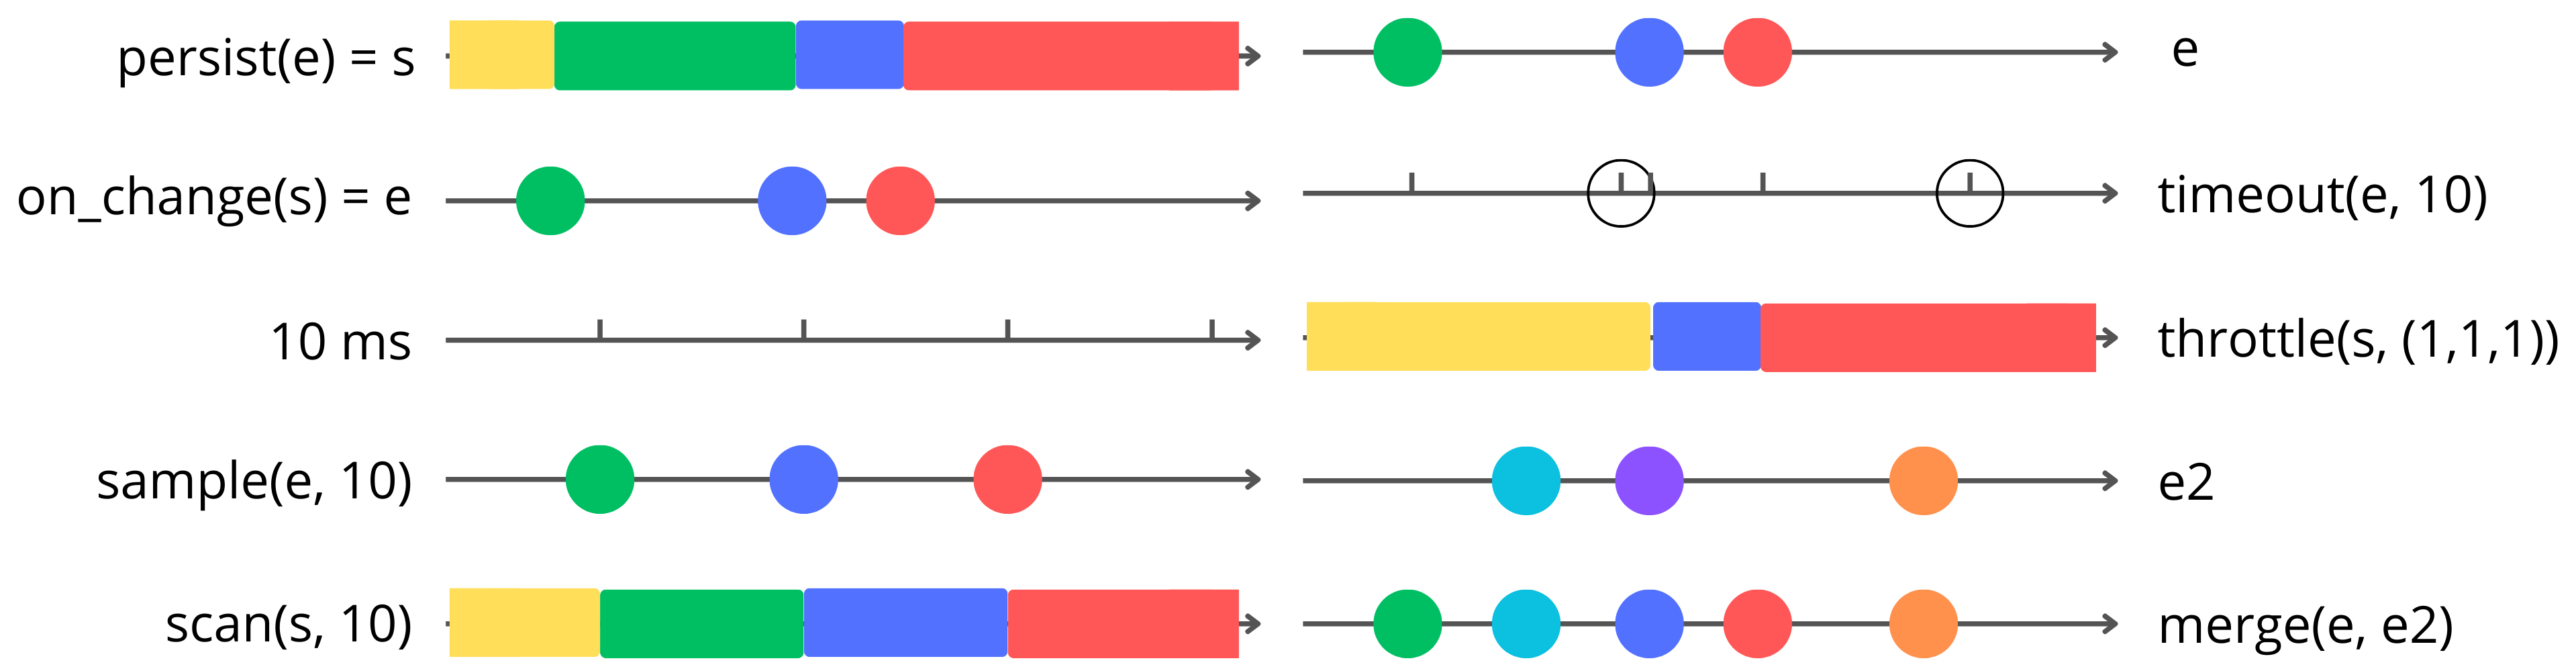
\includegraphics[width=\textwidth]{../images/greact.png}
    \caption[Chronograms of \GReact operators.]
    {Chronograms of \GReact operators (\texttt{10 ms} is used for \kft{sample} and \kft{scan}).}
    \label{fig:greact_operators}
\end{figure}

\subsection{Syntax of \GRSync}
\label{sec:grust:syntax:grsync}

This section presents \GRSync, a language for defining custom flow operators. Its syntax is shown in
EBNF notation in \Cref{fig:syntax:grsync}. \GRSync is highly inspired by \Lustre-like
languages~\cite{DBLP:conf/tase/ColacoPP17,DBLP:conf/hybrid/BourkeP13,DBLP:conf/emsoft/CohenGP12},
which bridge the gap between functional requirements and the implementation of critical systems.
These languages use \emph{clocks} to explicitly define when computations are performed. However,
correct usage of clocks often requires a deep understanding of the formal semantics of the language.
\GRSync omits explicit clocks and instead offers other constructs for filtering computations,
presented in the following paragraphs, that are tailored to needs in the automotive industry.

\begin{figure}[!ht]
    \centering
    \begin{bnf}(comment = {:is:})
        \FunItem ::= \funItem{\ID}{\many{(\ID \: \kft{:} \: \TY)}}{\TY}{\many{\Decl}} ;;
        \CompItem ::= \compItem{\ID}{\many{(\ID \: \kft{:} \: \STY)}}{\many{(\ID \: \kft{:} \: \STY)}}{\many{\Eq}} ;;
        \Eq ::= \Decl // \defEq{\many{\ID}}{\Expr} // \initEq{\ID}{\CST}
        | \matchX{\Expr}{\many{(\normBr{\gPat{\Pat}{\Expr}}{\setEq})}}
        | \whenEq{\initBr{\many{(\ID \: \kfm{=} \: \CST\kft{;})}}}{\many{(\normBr{\gPat{\EPat}{\Expr}}{\setEq})}} ;;
        \Decl ::= \declEq{\many{(\ID \: \kft{:} \: \STY)}}{\Expr} ;;
        \Expr ::= \CST // \ID // \lastExpr{\ID} // \emitExpr{\Expr} // \opExpr{\many{\Expr}} // \appExpr{\ID}{\many{\Expr}}
        | \matchX{\Expr}{\many{(\normBr{\gPat{\Pat}{\Expr}}{\Expr})}} ;;
        \Pat ::= \CST // \ID // \kft{\_} // \tuple{\Pat} ;;
        \EPat ::= \ID \kfm{=} \opt{\ID} // \Expr // \tuple{\EPat} ;;
        \STY ::= \TY // \opt{\TY} ;;
    \end{bnf}
    \caption[EBNF grammar of \GRSync.]%
    {EBNF grammar of \GRSync.
        Terminal symbols are in purple.
        Repetitions of \texttt{X} are denoted \many{\texttt{X}}.
        Option of \texttt{X} is denoted \texttt{X}?.
        \ID are identifiers composed of ASCII characters.
        \CST are constants.
        \OP represents $n$-ary operators (\eg addition).}
    \label{fig:syntax:grsync}
\end{figure}

User-defined flow operators are reusable building blocks, modeled as \emph{components} (\CompItem)
if they use a finite number of internal buffers, or as \emph{functions} (\FunItem) if they are
memory-free.

The signature of a component declares its name, and the sampling types and names of its input and
output flows.
%
The sampling type of a flow represents the type of the value present in that flow at any time.
For a signal \ID defined as \typed{\signalKind}{\ID}{\TY}, the sampling type is \TY as its value is
always present; for an event \ID defined as \typed{\eventKind}{\ID}{\TY}, the sampling type is the
option \opt{\TY} it might not have a value.
%
The body of a component is a set of mutually recursive equations (\setEq), stating the values
at every instant for the output flow based on the inputs. Ensuring that the output can be computed
at every time step is checked at compile-time, through an analysis called \emph{causality analysis}.
This is further explained in \Cref{sec:grust:implem:design_principles}.

The declaration of a function (\FunItem) is similar to that in traditional programming languages:
its signature declares a name, input flow names and types, and an output type. Its body contains an
ordered list of intermediary computations (\many{\Decl}) required to compute and return the output
(\kft{return} \Expr;). Functions operate on signal sampling types, as event handling typically
requires memory, which is reserved for components.

\GRSync offers the five kinds of equations that follow.
\begin{description}
    \item[Declaration] (\declEq{\many{(\ID:\STY)}}{\Expr}) defines local identifiers \many{\ID}.
    \item[Instantiation] (\defEq{\many{\ID}}{\Expr}) provides a definition for the outputs \many{\ID}.
    \item[Initialization] (\initEq{\ID}{\CST}) initializes a local signal \ID.
    \item[Match equation] (\matchX{\Expr}{\dots}) selects, for each instant, the first branch
          whose pattern (\Pat) matches the given expression and whose optional guard holds.
          Patterns can be constants, identifiers, wildcards, or tuples. Match equations must
          be exhaustive, ensuring a branch is always selected, and define the same identifiers.
    \item[When equation] (\whenEq{\initBr{\dots}}{\dots}) selects the first branch whose eventful
          pattern (\EPat) is satisfied and whose optional guard holds. An eventful pattern
          can be an event detection (\opt{\ID}), a rising edge detection (\Expr), or a
          conjunction of patterns. The activated branch performs punctual updates of signals
          and emissions of events. Signals not updated in a branch retain their previous
          values, which motivates their initialization in the \kft{init} branch.
\end{description}
Only declarations are used for intermediary computations in a function body.

Expressions are composed of constants (\CST), identifiers (\ID), $n$-ary operations
(\opExpr{\many{\Expr}}), component or function calls (\appExpr{\ID}{\many{\Expr}}), match
expressions (\matchX{\Expr}{\dots}), signal memories (\lastExpr{\ID}), and event emissions
(\emitExpr{\Expr}).

\subsection{Syntax of \GReusot}
\label{sec:grust:syntax:greusot}

\GRust enables formal verification by integrating with the \Creusot deductive verifier. This is
achieved through \GReusot, a language extension that allows developers to embed formal contracts
into \GRSync function and component declarations. The EBNF grammar governing these specifications is
detailed in \Cref{fig:syntax:greusot}.

\begin{figure}[!ht]
    \centering
    \begin{bnf}(comment = {:is:})
        \FunItem ::= \funItem[\Spec]{\ID}{\many{(\ID \: \kft{:} \: \TY)}}{\TY}{\many{\Decl}} ;;
        \CompItem ::= \compItem[\Spec]{\ID}{\many{(\ID \: \kft{:} \: \STY)}}
        {\many{(\ID \: \kft{:} \: \STY)}}{\many{\Eq}} ;;
        \Spec ::= \many{\Clause} ;;
        \Clause ::= \reqClause{\Term} // \ensClause{\Term} ;;
        \Term ::= \CST // \ID // \lastExpr{\ID} // \opExpr{\many{\Term}} // \tuple{\Term}
        // \appExpr{\ID}{\many{\Term}} | \implTerm{\Term}{\Term}
        // \forallTerm{\ID}{\TY}{\Term} | \whenTerm{\EPat}{\Term} // \resTerm ;;
    \end{bnf}
    \caption[EBNF grammar of \GReusot specifications.]{EBNF grammar of \GReusot specifications in component and function declarations.
        Terminal symbols are in purple. Repetitions of \texttt{X} are denoted \many{\texttt{X}}.
        \ID are identifiers. \CST are constants. \OP represents $n$-ary operators.}
    \label{fig:syntax:greusot}
\end{figure}

A specification (\Spec) is composed of one or more clauses (\Clause) that define preconditions
(\kft{requires}) and postconditions (\kft{ensures}). A precondition states the assumptions that must
be met for the function or component to execute correctly, while a postcondition describes the
properties that are guaranteed to hold upon completion.

These properties are expressed using logical terms (\Term). A term can be a constant (\CST), an
identifier (\ID), a reference to a past value (\lastExpr{\ID}), an $n$-ary operation
(\opExpr{\many{\Term}}), or a tuple (\tuple{\Term}). It can also represent a function call
(\appExpr{\ID}{\many{\Term}}), an implication (\implTerm{\Term}{\Term}), a universal quantifier
(\forallTerm{\ID}{\TY}{\Term}), or a conditional assertion based on an event
(\whenTerm{\EPat}{\Term}). For functions, the special term \resTerm refers to the return value.

\subsection{Summary}
This section has detailed the syntax of the \GRust language, which is structured around three core
elements and a proof extension. The high-level \GRFRP kernel is used to model asynchronous services
and define their external interfaces. The \GReact library provides a standard set of built-in
operators for common reactive patterns, inspired by \ReactiveX~\cite{reactivex}. For custom
operations, the \GRSync kernel offers a synchronous, equation-based language for defining stateful
components and stateless functions, using constructs like \texttt{when} and \texttt{match} for
controlled execution. Finally, the \GReusot extension integrates formal specification directly into
\GRSync, allowing developers to write contracts and prove critical properties. Together, these
elements form a comprehensive language for modeling, implementing, and verifying reactive systems.
